
\chapter{Language design}
When creating Giflang we had two options:
\begin{enumerate}
    \item Use a language with an existing web interpreter. 
    \item Create a new language and a web interpreter.
\end{enumerate}

In the first section of this chapter we explain why we decided to not reuse an existing language. Later, we discuss the design of our own language and
formally define it.

\section{Reusing an existing language}
In the previous chapter \ref{chap2} we concluded that interpreting the user code on the client-side is the best option for our project. Therefore, when
looking for a language to reuse we need to limit ourselves to the ones that have an existing web interpreter (i.e., an interpreter written in either
JavaScript or WebAssembly). The two major languages we considered reusing were Python and JavaScript.

\subsection{Python}
There are multiple Python web interpreters, for example Pyodide or Brython /TODO references/. Pyodide works by compiling CPython to WebAssembly
using Emscripten. On the other hand, Brython works by transpiling Python to JavaScript. We were not able to find a Python web interpreter that would
support code stepping out of the box. We considered forking either Pyodide or Brython and adding this functionality.

Adding code stepping to Pyodide would require changing the underlying CPython implementation. CPython is very complex and was not built for this use case and thus
we did opt out of choosing this option. On the other hand, Brython is fully written in JavaScript and also builds an AST from a Python code in JavaScript. There
is a fork of Brython /TODO ref/ that implements code stepping. However, at closer inspection we found out it runs the code all at once and records trace info at each
executed line by inserting a trace function call there. Afterwards, it only gives the user an illusion of code stepping.

It is possible to create a ``live'' code stepping for Brython in a similar fashion for example with the aid of Atomics API discussed in /TODO section/.
We did not find a simple way of increasing the stepping granularity from just lines, though. We definitely could have adjusted Brython instead
of creating a custom interpreter. However, it would take non-trivial effort to change the Brython's internals and we rather put this effort into creating
a new interpreter from scratch and learning a lot about languages and interpreters along the way.

\subsection{JavaScript}
There are numerous JavaScript interpreters written in JavaScript. The one closest to our needs being JS-Interpreter /TODO ref/ that supports running JavaScript
line by line in isolation. It was designed for use in Blockly /TODO ref/, a library for building visual programming editors.

JS-Interpreter supports only ES5\footnote{ECMAScript 5 or ECMAScript 2009} standard of JavaScript. This standard has no `class` keyword or block-scoping variables
with `let` keyword. We find ES5 way of defining classes using functions and prototypes confusing:
\begin{code}
// ES 5
function Person(name) {
    this.name = name;  
}

Animal.prototype.greet = function () {
    console.log('Hello my name is ' + this.name);
}

// ES 6
class Person {
    constructor(name) {
        this.name = name
    }

    greet() {
        console.log('Hello my name is ' + this.name);
    }
}
\end{code}

We could add support for ES6 features to the JS-Interpreter and use it for our project. However, as in the case of Brython we decided to rather put the effort into
creating a new solution than forking an existing one.

\section{Text format}
Before we dive into the language itself, let us first discuss the text representation of the language. Since it is intended for being displayed in
graphics using images we considered defining the language as semicolon delimited tokens where each token can be substituted with a single image.
Below is an identity function defined in both a character-level and a token-level format.
\begin{code}
// Token-level
FUNCTION; I;D; LPAR; A; RPAR; LCURLY;
RETURN; A; SEMICOLON;
RCURLY;

I;D; LPAR; 8; RPAR; SEMICOLON;

// Character-level
function ID(A) {
    return A;
}

ID(8);
\end{code}

We could just replace all characters of the character-level format with images, but keywords like ``function'' would result in multiple images. In the token-level
format we define function as a single token ``FUNCTION'' and is thus replaced with a single image.

In case of the character-level format we could replace everything character by character with images unless ``function'' or any other keyword is found in which
case we would replace it with a single image. However, it is not perfect. For example we should consider:
\begin{itemize}
    \item An identifier ``functionA'' should not have its ``function'' part replaced for an image.
    \item When an image for a keyword, e.g., ``function'' is used inside a string, it should be represented as a single character.
\end{itemize}

One possible solution is to represent keywords as single characters in the character-level format. This makes the image substitution trivial, as we can substitute
every character. The ``keyword characters'' have to be unique among other characters, though. For example we can use a Unicode letter `f' with a hook $f$
to represent a function and a character $\hookleftarrow$ for return.
\begin{code}
$f$ ID(A) {
    $\hookleftarrow$ A;
}

ID(8);
\end{code}

The above approach that uses Unicode characters has a nice property regarding the use of the keywords in a string. According to the ECMAScript specification,
Section 8.4/TODO cite/: When a String contains actual textual data, each element is considered to be a single UTF-16 code unit. This means that if we
only use characters that can be encoded into a single 16-bit code unit, all keywords will take space of a single character in a string.

At first we implemented the token-level format approach. It made parsing a little hard as typical lexer responsibilities like processing an identifier
had to be moved to the syntactical analysis. Later on we decided to switch to the character-level format with keywords substituted for Unicode characters. This
simplified the parsing.

\section{Deciding on a language type}
Now that we know we want to build our own language it is time to decide on what kind of language it should be and what features it should have. There are
multiple types of programming languages and here we will briefly go through the most known ones.

\subsection{Functional programming}
Functional programming treats computation as the evaluation of mathematical functions and avoids changing-state and mutable data.\footnote{wikipedia}
This means that functional programming languages don’t support imperative flow controls like loop statements, conditional statements like if-else and
switch statements.

On the other hand, pure functions are very typical for functional programming. Pure functions are functions whose outcome depends solely on their arguments
and create no side-effects (e.g., by changing a global variable). Eliminating side effects can make understanding a program easier, which is one of the
key motivations for the development of functional programming.\footnote{wiki}

Additionally, functional programming often relies on recursion and functions being first-class entities. Being a first-class entity means that functions can appear
anywhere in the program where other first-class entities like numbers can, including as arguments to other functions and as their return values.

One of the typical examples of a functional programming language is Haskell. It was created in 1990 and it is statically typed and supports type inference
and lazy evaluation. Below is a sample program in Haskell finding edit distance\footnote{} between two strings from the official docs.
\begin{code}
import Data.Array as Array

editDistance :: Eq a => [a] -> [a] -> Int
editDistance xs ys = table ! (m,n)
    where
    (m,n) = (length xs, length ys)
    x     = array (1,m) (zip [1..] xs)
    y     = array (1,n) (zip [1..] ys)
    
    table :: Array (Int,Int) Int
    table = array bnds [(ij, dist ij) | ij <- range bnds]
    bnds  = ((0,0),(m,n))
    
    dist (0,j) = j
    dist (i,0) = i
    dist (i,j) = minimum [table ! (i-1,j) + 1, table ! (i,j-1) + 1,
        if x ! i == y ! j
            then table ! (i-1,j-1)
            else 1 + table ! (i-1,j-1)]
\end{code}

\subsection{Object-oriented programing}
Object-oriented programming (OOP) is based around the concept of ``objects'', which can contain data, in the form of fields (also known as attributes or properties),
and code, in the form of methods.\footnote{wiki} Object's methods can access and modify the object they are operation using a keyword like ``this'' or ``self''.
Typical programs are then made out of objects that interact together.

The most popular OOP languages are class-based (e.g., C++, Java, Python), meaning that objects are instances of classes, which also determine their types.\footnote{wiki}
There are also alternatives, for example JavaScript is prototype-based.

OOP has a few features that are common among most of the object-oriented programming languages:
\begin{itemize}
    \item Inheritance or subclassing lets developers create a new class by building upon an existing one.
    \item Encapsulation allows hiding data and methods of an object from the outside interference and misuse.
    \item Polymorphism allows calling code to be agnostic as to which class in the supported hierarchy it is operating on.
\end{itemize}

Below is an example of polymorphism in C++.
\begin{code}
class Animal {
public:
    Animal() : { }
    virtual string make_sound() = 0;
};

class Dog: public Animal {
public:
    Dog() : Animal() { }
      
    string make_sound() { 
        return "Woof, woof!"; 
    }
};

class Sheep: public Animal {
public:
    Sheep() : Animal() { }
      
    string make_sound() { 
        return "Baa, baa!"; 
    }
};

int main() {
    Animal *animal;
    Dog dog();
    Sheep sheep();

    // Store the address of Dog.
    animal = &dog;

    // Call Dog's make_sound. Returns "Woof, woof!".
    animal->make_sound();

    // A similar example with sheep. Returns "Baa, baa!".
    animal = &sheep;
    animal->make_sound();

    return 0;
}
\end{code}

\subsection{Esoteric programming languages}
An esoteric programming language is designed to experiment with weird ideas, to be hard to program in, or as a joke, rather than for practical use. We can not
describe esoteric languages in general as they all use different ideas. However, we will show a few examples of esoteric languages.

Probably the most popular esoteric language is brainf***. It operates on an array of memory cells, also referred to as the tape. All of the cells are initially
set to zero. There is a single pointer, initially pointing to the first memory cell. The language has the following commands:

\begin{figure}[!hbt]
    \centering
    \begin{tabular}{|c l |} 
    \hline
    $>$ & Move the pointer to the right \\
    \hline
    $<$ & Move the pointer to the left \\
    \hline
    $+$ & Increment the memory cell under the pointer \\
    \hline
    $-$ & Decrement the memory cell under the pointer \\
    \hline
    $.$ & Output the character signified by the cell at the pointer \\
    \hline
    $,$ & Input a character and store it in the cell at the pointer \\
    \hline
    $[$ & Jump past the matching ] if the cell under the pointer is 0 \\
    \hline
    $]$ & Jump back to the matching [ if the cell under the pointer is nonzero \\
    \hline
    \end{tabular}
    \caption{The list of brainf*** commands}
\end{figure}

Other examples of esoteric languages:
\begin{itemize}
    \item Shakespeare /TODO ref/, a programming language whose source code resembles Shakespeare plays. 
    \item Befunge /TODO ref/, a language where the code is layed out on a two-dimensional grid of instructions, and execution can proceed in any direction of that grid.
\end{itemize}

\subsection{Conclusion}
There are also other programming types for example logic programming. However, we did not plan on using concepts from these languages and therefore we did
not explain them here. It would be great to combine a language presented in images with an esoteric language of some sort. However, we did not
come up with an interesting enough model and we did not want to blindly reuse an existing one. Therefore, we settled on a more conservative approach.

Since our intended audience is typically experienced in Python we decided to base our language around "Pythonic" features. We also think
the class-based model of Python is more intuitive than prototype-based one found for example in JavaScript.

Even though the author of this thesis likes statically-typed languages, Giflang is dynamically-typed. The primary reason is that the images take a lot of
space on the user screen and hence we tried to keep the language concise. Adding typed declarations would probably make it less error-prone, but more verbose.

\section{Object model}
As mentioned in the end of the previous section we base Giflang on Python. Everything is an object in Python. An object A can have multiple
related objects:
\begin{itemize}
    \item An instance B that denotes the type of A. We call B a \texttt{klass} of the instance A and we say that A is an instance of B.
    \item If A is a class (i.e., an instance of MetaClass), it can have multiple base classes. These base classes are just another Python objects. Let B denote
    one of the base classes. We then say that A derives from B. 
\end{itemize}

As the Figure \ref{fig:chap3:python_structure} shows classes are instances of a MetaClass and the MetaClass is an instance of itself.

\begin{figure}[!hbt]
    \centering
    \tikzset{every picture/.style={line width=0.75pt}} %set default line width to 0.75pt        
    \trimbox{0cm .75cm 0cm 0cm}{
        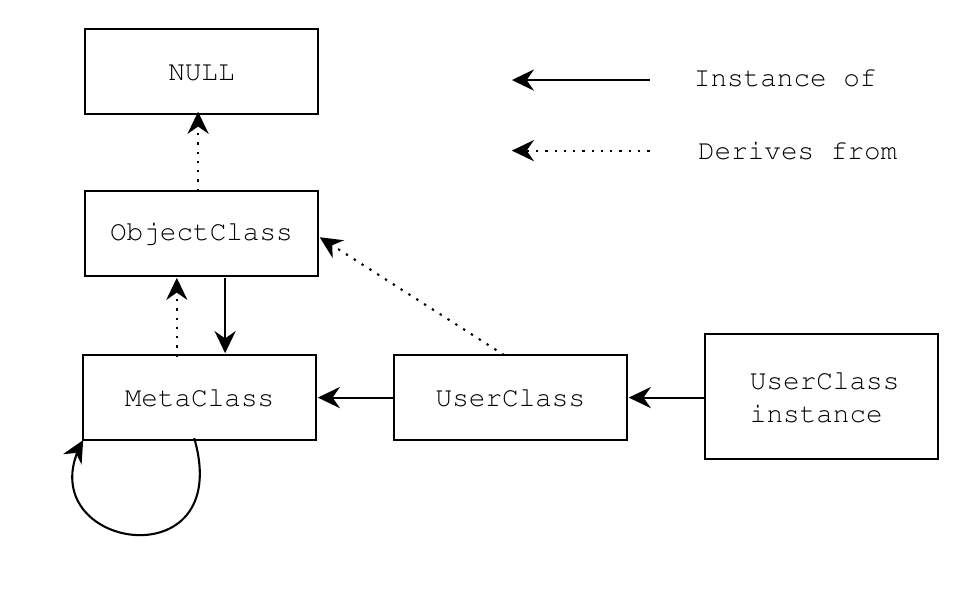
\begin{tikzpicture}[x=0.75pt,y=0.75pt,yscale=-1,xscale=1]
        \draw   (13.61,159.25) -- (125.73,159.25) -- (125.73,200.19) -- (13.61,200.19) -- cycle ;
        \draw    (67.11,199.26) .. controls (87.27,268.92) and (-12.63,252.81) .. (12.38,202.52) ;
        \draw [shift={(13.61,200.19)}, rotate = 479.36] [fill={rgb, 255:red, 0; green, 0; blue, 0 }  ][line width=0.08]  [draw opacity=0] (10.72,-5.15) -- (0,0) -- (10.72,5.15) -- (7.12,0) -- cycle    ;
        \draw   (14.54,80.16) -- (126.66,80.16) -- (126.66,121.1) -- (14.54,121.1) -- cycle ;
        \draw  [dash pattern={on 0.84pt off 2.51pt}]  (58.73,160.18) -- (58.73,129.48) -- (58.73,125.03) ;
        \draw [shift={(58.73,122.03)}, rotate = 450] [fill={rgb, 255:red, 0; green, 0; blue, 0 }  ][line width=0.08]  [draw opacity=0] (10.72,-5.15) -- (0,0) -- (10.72,5.15) -- (7.12,0) -- cycle    ;
        \draw   (14.54,2) -- (126.66,2) -- (126.66,42.94) -- (14.54,42.94) -- cycle ;
        \draw  [dash pattern={on 0.84pt off 2.51pt}]  (68.97,80.16) -- (68.97,49.45) -- (68.97,45.01) ;
        \draw [shift={(68.97,42.01)}, rotate = 450] [fill={rgb, 255:red, 0; green, 0; blue, 0 }  ][line width=0.08]  [draw opacity=0] (10.72,-5.15) -- (0,0) -- (10.72,5.15) -- (7.12,0) -- cycle    ;
        \draw    (82,122.03) -- (82,155.32) ;
        \draw [shift={(82,158.32)}, rotate = 270] [fill={rgb, 255:red, 0; green, 0; blue, 0 }  ][line width=0.08]  [draw opacity=0] (10.72,-5.15) -- (0,0) -- (10.72,5.15) -- (7.12,0) -- cycle    ;
        \draw   (163.41,159.25) -- (275.54,159.25) -- (275.54,200.19) -- (163.41,200.19) -- cycle ;
        \draw    (162.95,179.72) -- (129.66,179.72) ;
        \draw [shift={(126.66,179.72)}, rotate = 360] [fill={rgb, 255:red, 0; green, 0; blue, 0 }  ][line width=0.08]  [draw opacity=0] (10.72,-5.15) -- (0,0) -- (10.72,5.15) -- (7.12,0) -- cycle    ;
        \draw  [dash pattern={on 0.84pt off 2.51pt}]  (216.45,159.25) -- (130.12,104.11) ;
        \draw [shift={(127.59,102.49)}, rotate = 392.57] [fill={rgb, 255:red, 0; green, 0; blue, 0 }  ][line width=0.08]  [draw opacity=0] (10.72,-5.15) -- (0,0) -- (10.72,5.15) -- (7.12,0) -- cycle    ;
        \draw   (313.22,149.02) -- (425.35,149.02) -- (425.35,209.5) -- (313.22,209.5) -- cycle ;
        \draw    (312.76,179.72) -- (279.47,179.72) ;
        \draw [shift={(276.47,179.72)}, rotate = 360] [fill={rgb, 255:red, 0; green, 0; blue, 0 }  ][line width=0.08]  [draw opacity=0] (10.72,-5.15) -- (0,0) -- (10.72,5.15) -- (7.12,0) -- cycle    ;
        \draw    (286.5,26.74) -- (223.15,26.74) ;
        \draw [shift={(220.15,26.74)}, rotate = 360] [fill={rgb, 255:red, 0; green, 0; blue, 0 }  ][line width=0.08]  [draw opacity=0] (10.72,-5.15) -- (0,0) -- (10.72,5.15) -- (7.12,0) -- cycle    ;
        \draw  [dash pattern={on 0.84pt off 2.51pt}]  (286.5,60.74) -- (223.15,60.74) ;
        \draw [shift={(220.15,60.74)}, rotate = 360] [fill={rgb, 255:red, 0; green, 0; blue, 0 }  ][line width=0.08]  [draw opacity=0] (10.72,-5.15) -- (0,0) -- (10.72,5.15) -- (7.12,0) -- cycle    ;
        \draw (69.67,179.72) node   [align=left] {{\fontfamily{pcr}\selectfont MetaClass}};
        \draw (70.6,100.63) node   [align=left] {{\fontfamily{pcr}\selectfont ObjectClass}};
        \draw (70.6,23.4) node   [align=left] {{\fontfamily{pcr}\selectfont NULL}};
        \draw (219.48,179.72) node   [align=left] {{\fontfamily{pcr}\selectfont UserClass}};
        \draw (370.87,179.72) node   [align=left] {{\fontfamily{pcr}\selectfont  UserClass}\\{\fontfamily{pcr}\selectfont instance}};
        \draw (351.87,25.72) node   [align=left] {{\fontfamily{pcr}\selectfont Instance of}};
        \draw (357.87,60.72) node   [align=left] {{\fontfamily{pcr}\selectfont Derives from}};
        \end{tikzpicture}
    }
    \caption{Object structure in Python.}
	\label{fig:chap3:python_structure}
\end{figure}

MetaClass is actually called \texttt{type} in Python. Below is an interactive Python session that unveils the internals of Python shown in the
Figure \ref{fig:chap3:python_structure}.
\begin{code}
>>> class X:
...     pass
... 
>>> type(X)
<class 'type'>
>>> x = X()
>>> type(x)
<class '__main__.X'>
>>> x.__bases__
Traceback (most recent call last):
  File "<stdin>", line 1, in <module>
AttributeError: 'X' object has no attribute '__bases__'
>>> type(type(X))
<class 'type'>
>>> type(X).__bases__
(<class 'object'>,)
>>> type(type(X).__bases__[0])
<class 'type'>
\end{code}

We decided to reuse this model as the base of Giflang. Another Python feature we reused are magic methods as they provide a very straightforward way
to overload operators. Magic methods are prefixed and suffixed with two underscores. Below is a Python example that uses magic methods:
\begin{code}
class Number:
    # Defines a constructor
    def __init__(self, val):
        self.val = val
    
    # Defines a string representation
    def __str__(self):
        return str(self.val)

    # Overloads operator +
    def __add__(self, other):
        return Number(self.val + other.val)

    # Overloads a call operator
    def __call__(self):
        return 'An instance was called :)'

x = Number(2)
y = Number(3)
# Outputs 5. First __add__ is called and then __str__ on the result.
print(x + y)
# Outputs 'An instance was called :)'
print(x())
\end{code}

The example shows how to create a constructor, overload an operator and create a new instance of a class by calling the class with arguments for the constructor.
Number class also defines a \texttt{\_\_call\_\_} method so naturally we might expect the call \texttt{Number(2)} to result in the string `An instance was called :)'. However,
as we know, it is not the case. Instead, \texttt{Number(2)} results in a new instance of the Number class. The author of this thesis thinks that this is
the reason why magic method resolution in Python starts from the instance type rather than from the instance itself, as it is the case with regular methods.

Following up on the idea from the previous paragraph, because the call \texttt{Number(2)} does not result in the call of the \texttt{\_\_call\_\_} function on the
\texttt{Number} type, it has to result in a \texttt{\_\_call\_\_} method further up the chain. In this case, \texttt{Number} is an instance of the \texttt{type},
or the MetaClass class. Its \texttt{\_\_call\_\_} method is responsible for creating a new instance and calling the \texttt{\_\_init\_\_} method. Oversimplified,
the \texttt{type}'s \texttt{\_\_call\_\_} function might look like this:
\begin{code}
class type:
    # Since classes are instances of the 'type' class, self
    # in this method is the class object. 
    def __call__(self, *args, **kwargs):
        obj = instantiate(self)
        obj.__init__(*args, **kwargs)
        return obj
\end{code}

In reality, creating a new instance is a little more complicated, To give users more control over the instantiation, another magic method \texttt{\_\_new\_\_}
is called instead of a made up function \texttt{instantiate} in the example above. We did not go into more detail since we decided to not include the
\texttt{\_\_new\_\_} magic method into Giflang as it is mainly used only for a few specific use cases (e.g., creating a singleton).

Having a keyword for introducing new variables, e.g., \texttt{var}, would mean that magic methods could be resolved the same way as normal methods. However,
we like the simplicity of creating a new instance via calling a class and therefore used this approach in Giflang as well.

\section{Flow constructs}
Giflang supports basic flow constructs: \texttt{if}, \texttt{while} and \texttt{for}. The author of this thesis is a fan of C-like \texttt{for} and therefore


\section{Native types}
